\chapter{Arquitectura}
\label{chap:architecture}


\section{Introducción}
\label{sec:introduction}

En este capítulo trataremos la fase de diseño de este proyecto, así como los detalles de implementación de dicha arquitectura. Primero, presentaremos una vista general del proyecto por medio de un escenario. A continuación se mostrará la arquitectura en el cliente, así como la del servidor y los servicios que la componen. Posteriormente, se detallarán los módulos que conforman la aplicación, así como las métricas que se han decidido calcular y sus motivos. Con ello tenemos la intención de facilitar al lector una vista general de la arquitectura del proyecto.

Se presenta a continuación el escenario principal de uso de ChatStats:

\begin{figure}[H]
	\centering
	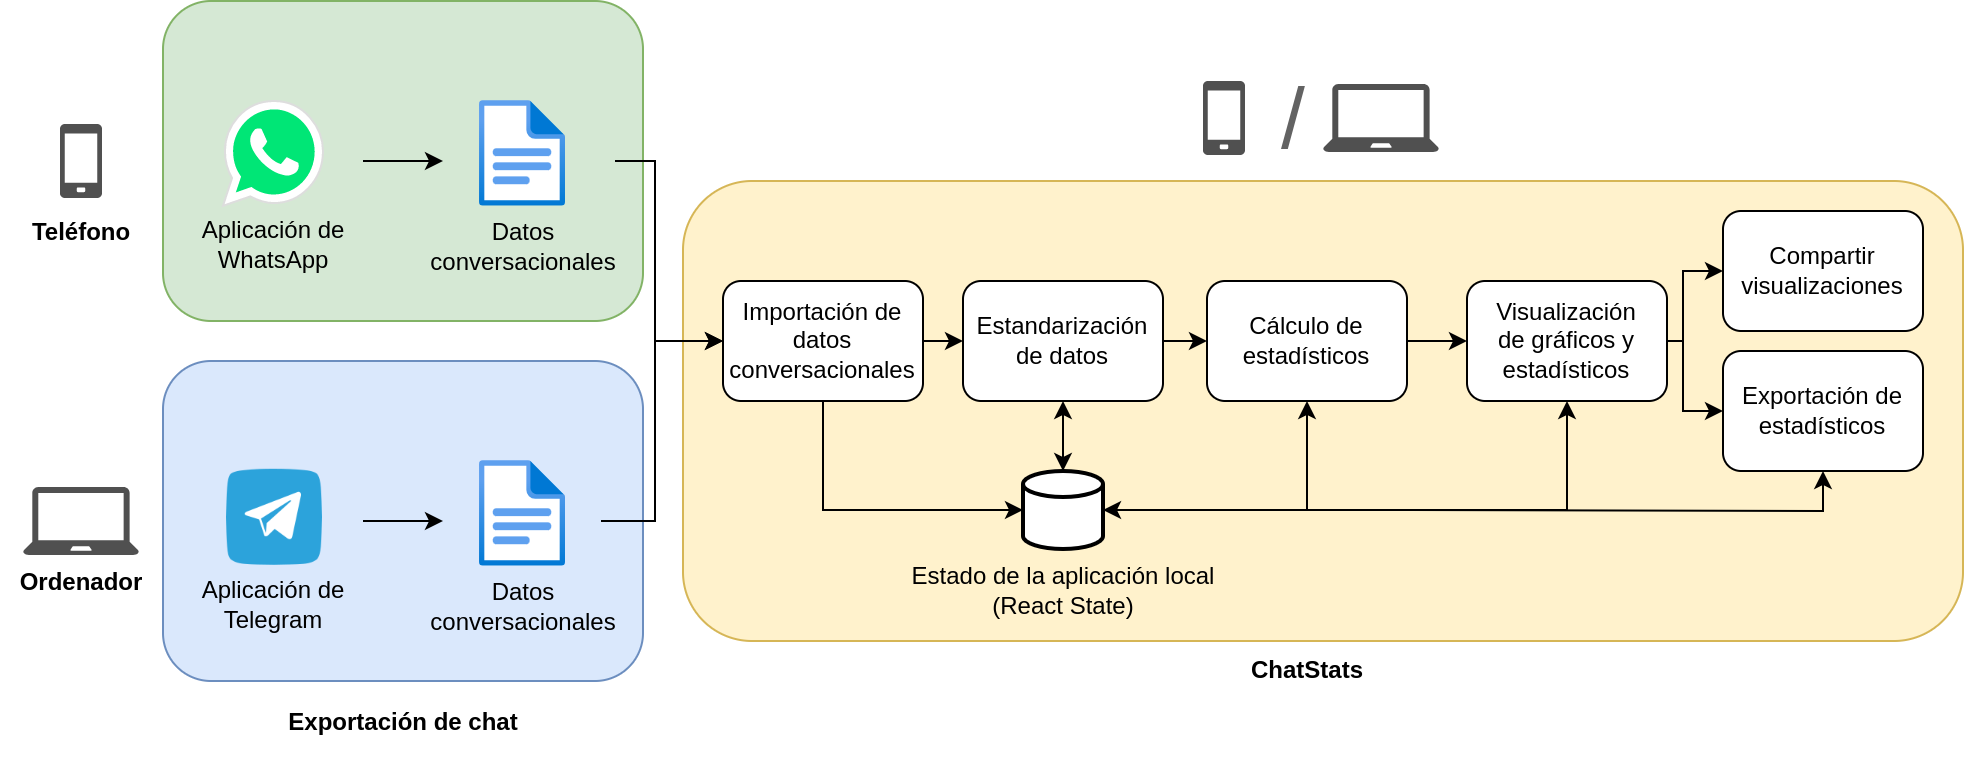
\includegraphics[width=\textwidth]{img/scenario.png}
	\caption{Escenario de ChatStats}
	\label{fig:chap4:architecture_scenario}
\end{figure}

\todi{El servidor únicamente sirve la página... ¿Debería meterlo aquí? ¿Cómo?}

\section{Arquitectura de procesamiento}
\label{chap:architecture:processing}




Para mantener la privacidad de los datos del usuario, se ha planteado las siguientes opción de diseño:

El cliente solicita la aplicación, que se envía en su totalidad.

La primera, y más segura, es que los datos nunca salgan del dispositivo de ninguna forma. Esto supondrá coste computacional en el cliente para realizar las operaciones necesarias, por lo que el código deberá ser altamente eficiente. En este caso, el cliente descargaría toda la aplicación web en una petición (y sus consecuentes). Tras ello, ningún dato se enviaría al servidor.

La segunda forma implica el desarrollo de lógica de negocio en un servidor, también de código libre, que no almacene datos en el disco duro, realizando todas las operaciones en la memoria volátil. Este servidor no debería tener ningún tipo de trazas de las operaciones y debería usar un protocolo de comunicación seguro como \acrfull{https}. Como punto positivo, el servidor contaría con mayor capacidad de computación que el cliente, permitiendo mayor velocidad en las operaciones o una mayor complejidad de las mismas.

Se plantea también una tercera opción, que consiste en el híbrido de las primeras dos opciones. En este caso, el cliente puede realizar todas las operaciones en local y, activando un interruptor en la aplicación, puede optar a mandar sus datos a un servidor externo para realizar funciones más avanzadas y obtener más información.

Por el momento, hemos comenzado con la primera implementación, puesto que se considera fácilmente extensible hacia la tercera opción, con un modelo de ejecución en cliente con opción a realizar procesamiento de algunas funciones en un servidor.

A continuación se muestra la arquitectura de la lógica de negocio:

\begin{figure}[H]
	\centering
	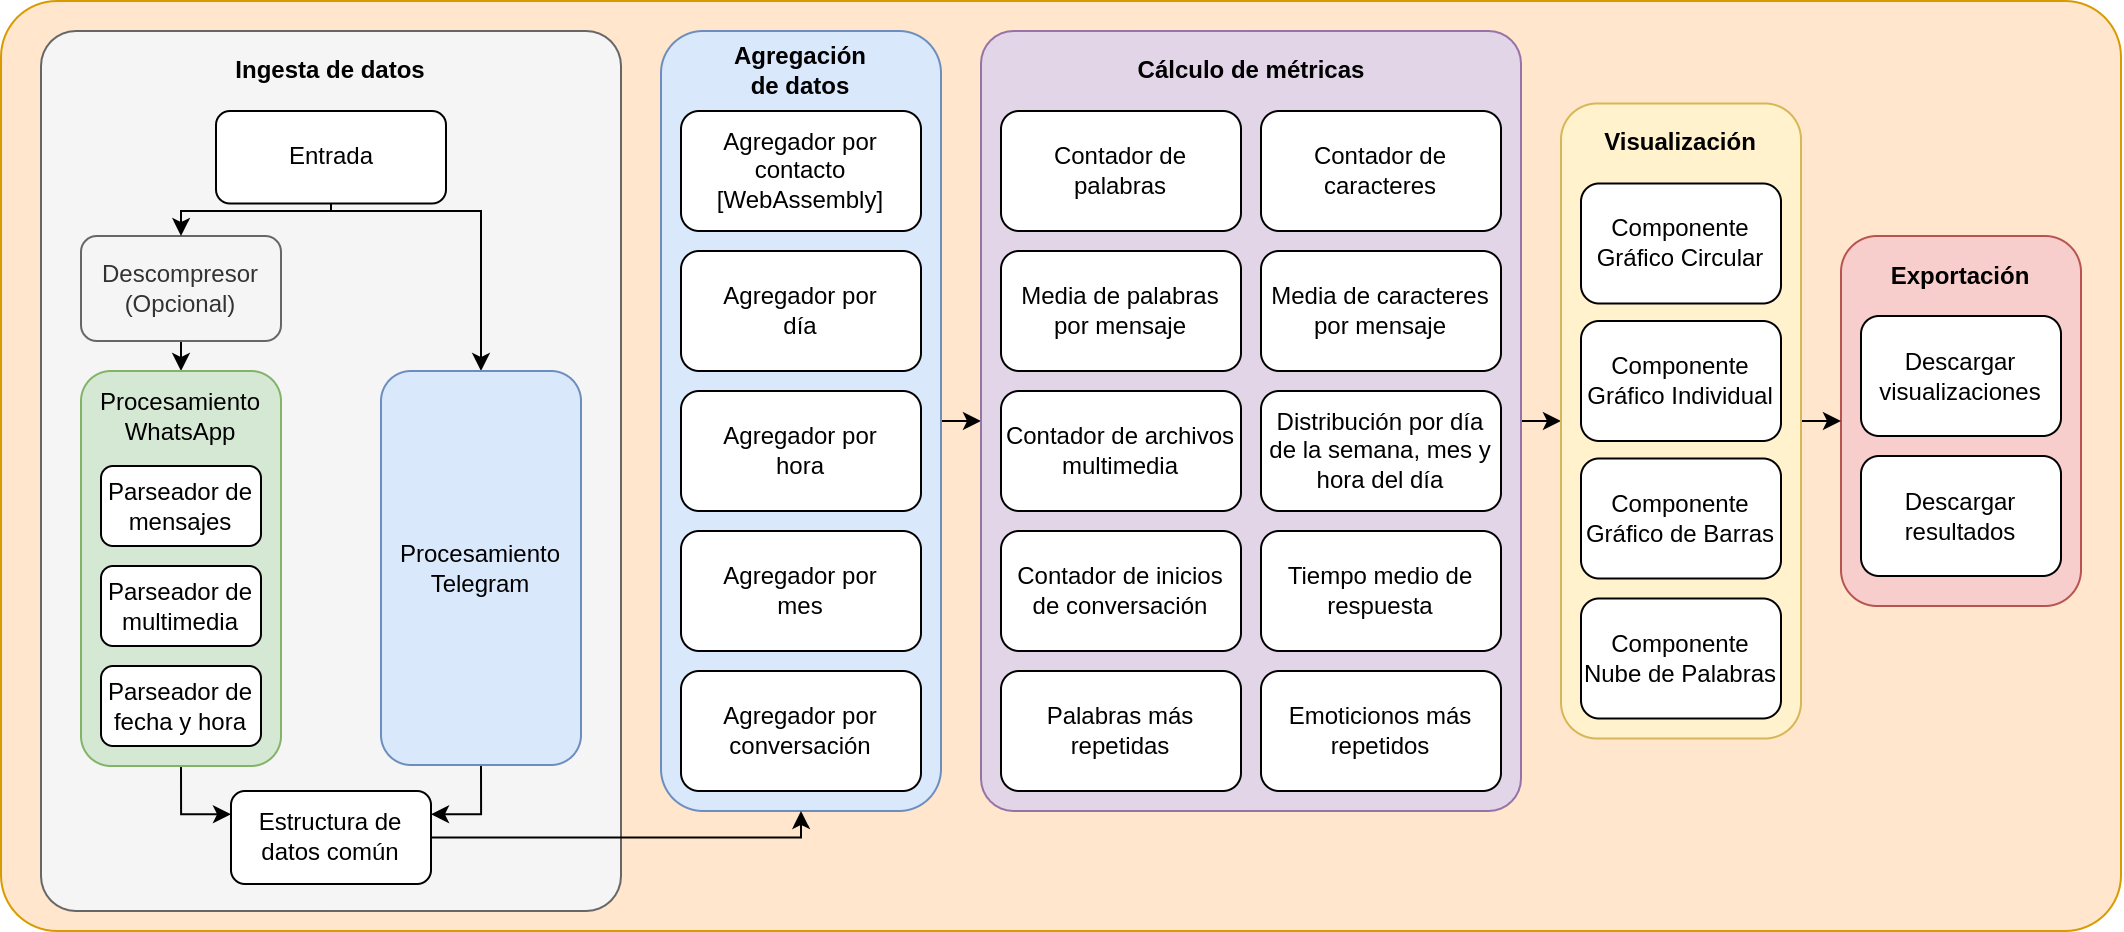
\includegraphics[width=\textwidth]{img/architecture_processing.png}
	\caption{Arquitectura de procesamiento}
	\label{fig:chap4:architecture_processing}
\end{figure}

\todi{Corregir Analyser a Aggregators}

\subsection{Input}

Se trata de un conjunto de funciones que acceden y leen el archivo de entrada que el usuario ha proporcionado. Este archivo puede ser en texto plano o comprimido, como se explica en el siguiente módulo.

\subsection{Descompresor (Opcional)}

Mientras que en los sistemas operativos Android, la aplicación WhatsApp exporta los chats en texto plano, en los sistemas operativos iOS se exportan en un archivo comprimido en formato \textit{zip}. En este último caso, dentro del archivo se encuentra un fichero denominado \textit{\_chat.txt}, junto con el resto de contenido multimedia (fotos, vídeos y documentos) en caso de haber optado por exportarlos.

Este módulo descomprime el archivo en el cliente y se queda únicamente con el fichero \textit{\_chat.txt}, que contiene toda la información necesaria para el análisis.

\subsection{Parser}

Este módulo se compone de diferentes submódulos para parsear los diferentes tipos de objetos contenidos en cada grupo de la cadena de texto.

Todo comienza por encontrar una expresión regular que pueda buscar coincidencias en el archivo de texto, así como dividir estas coincidencias en los grupos correspondientes. Tras analizar varias fuentes de datos con distintos dispositivos, hemos detectado que existen dos formatos de mensaje: uno para Android y otro para dispositivos iOS.

A continuación se muestra un mensaje en el formato de los dispositivos Android como ejemplo:

\begin{lstlisting}
	17/07/2022, 01:28 - Alice: Este es un mensaje de prueba
\end{lstlisting}

También se muestra un mensaje exportado por un dispositivo iOS:

\begin{lstlisting}
	[29/12/22, 0:14:55] Bob: Te escribo desde mi iPhone.
\end{lstlisting}

Podemos observar que ambos mensajes se componen de la fecha, la hora, el nombre del contacto y el propio cuerpo del mensaje, aunque con distinto formato.

Para poder separar cada mensaje se ha llegado a la siguiente expresión regular:

\begin{lstlisting}
	/\[*(\d{1,2}\/\d{1,2}\/\d{2,4}),\s(\d{1,2}:\d{2}:*\d*)\]*\s(?:-\s)*(.*?):{1}\s(.*?)(?=\s\[*\d{1,2}\/\d{1,2}\/\d{2,4}|$)/gum
\end{lstlisting}

Los grupos de captura que lo componen se describen en detalle en el \autoref{chap:regex}.

\todi{Actualizar grupos de captura con los de iPhone}


\subsubsection{Parser de cadenas de caracteres de tiempo}

Este submódulo recoge las coincidencias del grupo de captura 1 y 2, devolviendo un objeto de tipo \textit{Date}, lo cual nos permitirá operar con el fácilmente. Este módulo considera el \textit{locale} del cliente, invirtiendo mes y día para el caso \textit{en\_US}.

Asimismo, el módulo considera los posibles formatos de fecha y hora, puesto que en iOS se incluyen los segundos y se usan los días, meses y horas sin cero a la izquierda; contrario a Android.

\subsubsection{Parser de archivos multimedia}

Existen dos opciones para exportar un chat: con contenido multimedia o sin él.

\paragraph{Con contenido multimedia}\mbox{}\\

En el primer caso, WhatsApp exporta el fichero de texto plano, además de todas las imágenes, vídeos, música, notas de voz o documentos del chat. En caso de iOS, todos los archivos se agrupan en un archivo comprimido en \textit{zip}, mientras que en Android se exportan todos los archivos como individuales, permitiendo al usuario compartirlos con la aplicación deseada (o guardarlos).

En un mensaje con contenido multimedia, observaremos que el cuerpo incluirá el nombre del fichero que se ha exportado con la extensión del formato del mismo. Por ello, categorizamos como \textit{voice\_message}, \textit{video\_file}, \textit{sticker} o \textit{image} en función a la extensión; \textit{.opus}, \textit{.mp4}, \textit{.webp} o \textit{.jpg}, respectivamente.

Se indican a continuación mensajes de ejemplo para cada tipo de archivo adjunto, únicamente para Android:

\begin{lstlisting}
	17/10/2022, 21:11 - Juan Pedro: PTT-20221017-WA0078.opus (file attached)
	20/10/2022, 10:37 - Juan Pedro: IMG-20221020-WA0013.jpg (file attached)
	14/11/2022, 18:58 - Juan Pedro: VID-20221114-WA0039.mp4 (file attached)
	24/11/2022, 19:13 - Jaime Conde: STK-20220717-WA0090.webp (file attached)
\end{lstlisting}

\paragraph{Sin contenido multimedia}\mbox{}\\

Para el segundo caso, cada vez que un mensaje sea contenido multimedia, aparecerá \textit{\textless Media omitted \textgreater} (multimedia omitido). Estos pueden ser fotos, vídeos, música, notas de voz o documentos. Se definirán como \textit{undefined} o indefinidos, ignorándose en las visualizaciones y módulos posteriores.

\begin{lstlisting}
	17/07/2022, 01:33 - Juan Pedro: <Media omitted>
\end{lstlisting}

\subsubsection{Parser de mensajes}

Este módulo convierte las cadenas de textos en un objeto \acrshort{json} con la siguiente estructura:

\begin{lstlisting}[language=JavaScript]
	{
		date: new Date("2022-10-17T10:37:00"),
		from: "Juan Pedro",
		text: "IMG-20221020-WA0013.jpg",
		type: "message",
		media_type: "image"
	}
\end{lstlisting}

En caso de tratarse de un mensaje de texto (no multimedia), el ``\textit{media\_type}'' será \textit{undefined} (indefinido) y ``\textit{text}'' contendrá el cuerpo del mensaje.

Serán estos los objetos que se utilizarán más adelante para calcular las estadísticas y las estructuras de datos de visualización.

\subsection{Agregadores}

Los mensajes se encuentran segregados en una lista, por lo que a continuación, el módulo de agregador se encargará de agregar los mensajes en diferentes grupos. En el código los hemos llamado polarizadores. Se describen los distintos submódulos a continuación:

\subsubsection{Agregador por contacto}

\textit{ChatStats} se encarga de calcular las estadísticas de cada contacto para visualizarlas y mostrarlas en comparación con el resto de contactos. Hablamos de numerosos contactos, puesto que es compatible con chats individuales y grupales.

El resultado de este submódulo será un objeto \acrshort{json} con una clave por cada contacto (su nombre), que contendrá un array de los mensajes enviados por este. Se indica un ejemplo:

\begin{lstlisting}[language=JavaScript]
	{
		"Jaime": [...messagesByJaime],
		"Juan Pedro": [...messagesByJuanPedro],
		...
	}
\end{lstlisting}

donde los array de mensajes contienen objetos definidos en el \textit{Parser de mensajes}.

\subsubsection{Agregador por día}

Este agregador toma como entrada la salida del submódulo anterior: los mensajes agregados por contacto. Con ello se procede a agregarlos, además, por día de la semana: de lunes a domingo. Se usará el nombre del día de la semana como clave anidada.

El resultado son objetos con la siguiente estructura:

\begin{lstlisting}[language=JavaScript]
	{
		"Jaime": {
			"monday": [...messagesByJaimeOnMonday],
			"tuesday": [...messagesByJaimeOnTuesday],
			...,
			"sunday": [...messagesByJaimeOnSunday]
			},
		"Juan Pedro": {
			"monday": [...messagesByJuanPedroOnMonday],
			"tuesday": [...messagesByJuanPedroOnTuesday],
			...,
			"sunday": [...messagesByJuanPedroOnSunday]
		},
		...
	}
\end{lstlisting}

El objetivo de esta estructura de datos es visualizar la distribución de los mensajes a lo largo de la semana, en media.

\begin{comment}
	Se deja para futuras líneas un gráfico en el que se pueda elegir el año a analizar, o un scroll vertical por años.
\end{comment}

\subsubsection{Agregador por hora}

Este agregador toma también como entrada los mensajes agregados por contacto. Con ello se procede a agregarlos, además, por hora del día, usando la hora en formato 24 horas como clave anidada de agregación: de 00 a 23 horas.

El resultado son objetos con la siguiente estructura:

\begin{lstlisting}[language=JavaScript]
	{
		"Jaime": {
			"00": [...messagesByJaimeAt00],
			"01": [...messagesByJaimeAt01],
			...,
			"23": [...messagesByJaimeAt23]
		},
		"Juan Pedro": {
			"00": [...messagesByJuanPedroAt00],
			"01": [...messagesByJuanPedroAt01],
			...,
			"23": [...messagesByJuanPedroAt23]
		},
		...
	}
\end{lstlisting}

El objetivo de esta estructura de datos es visualizar la distribución de los mensajes a lo largo del día, en media.

\subsubsection{Agregador por mes}

Este agregador toma también como entrada los mensajes agregados por contacto. Con ello se procede a agregarlos, además, por MM/YYYY, por lo que deja de tratarse de un agregador acotado: pueden haber tantas claves anidadas como meses se haya hablado.

El resultado son objetos con la siguiente estructura:

\begin{lstlisting}[language=JavaScript]
	{
		"Jaime": {
			"10/2022": [...messagesByJaimeOnOctober2022],
			"11/2022": [...messagesByJaimeOnNovember2022],
			...
		},
		"Juan Pedro": {
			"10/2022": [...messagesByJuanPedroOnOctober2022],
			"11/2022": [...messagesByJuanPedroOnNovember2022],
			...
		},
		...
	}
\end{lstlisting}

El objetivo de esta estructura de datos es visualizar la distribución de los mensajes a lo largo del tiempo, con una agregación mensual.

\subsection{Visualizador}

\todi{Añadir descripción emoji regex y emoji cloud}

Este módulo prepara los datos para ser representados por la librería de visualización elegida: \textit{ChartJS}. Además, también se procesan datos para otras librerías de visualización, como las nubes de palabras o \textit{word clouds}.

\subsubsection{Contador de palabras}

Este submódulo cuenta las palabras que hay en los mensajes de cada contacto y calcula la suma total de las mismas, obteniendo el número de palabras totales enviadas por cada contacto.

\subsubsection{Contador de caracteres}

Este submódulo cuenta los caracteres que hay en los mensajes de cada contacto y calcula la suma total de los mismos, obteniendo el número de caracteres totales enviados por cada contacto.

\subsubsection{Media de palabras por mensaje}

Este submódulo devuelve el número medio de palabras por mensaje para cada contacto.

\subsubsection{Media de caracteres por mensaje}

Este submódulo devuelve el número medio de caracteres por mensaje para cada contacto.

Tanto el número de caracteres como el número de palabras suelen indicar la misma información respecto a qué contacto escribe más.

\subsubsection{Contador de multimedia}

En caso de que existan objetos \acrshort{json} con el campo ``\textit{media\_type}'' distinto de \textit{undefined}, este módulo contará cuántos archivos multimedia de cada tipo ha mandado cada contacto.

\subsubsection{Contador de palabras más repetidas}

Este módulo elimina las palabras más comunes del español y el inglés, así como otros mensajes que WhatsApp añade, como \textit{Media ommited} o \textit{This message has been deleted}.

Las listas de palabras más comunes del español e inglés se han recopilado de distintas fuentes, combinado y eliminado repeticiones.

A la salida de este módulo, se entrega un diccionario con las palabras más repetidas y el número de veces que aparece cada una; información de la que hará uso la nube de palabras.

\todi{Añadir fuzzy-wuzzy (se ha usado fuzzball)... Debería añadirlo a las tecnologías habilitantes?}

\todi{Anexar enlace a listas de palabras más comunes en anexo C}

% Contar que es para hacer un word cloud y que se eliminan las palabras más comunes del lenguaje inglés y español. También se deben eliminar enlaces, Media ommitted y This message has been deleted. Añadir fuzzywuzzy a la arquitectura del sistema (esquema) y al código.

% Contar de dónde se han recopilado las listas de palabras más comunes y anexar en C, junto con el código.

% Añadir fuzzy-wuzzy a las tecnologías habilitantes?

\subsubsection{Contador de emoticonos más usados}

Este módulo aplica una expresión regular unicode a todos los mensajes, seleccionando los emoticonos y contando el número de veces que aparecen. Posteriormente otra nube de palabras hará uso de esta información.

\subsubsection{Generador de estructuras de datos por día, hora y mes}

Para el gráfico de barras con el número de mensajes en el tiempo, \textit{ChartJS} necesita una estructura de datos para mensajes por día, siendo los días la variable independiente y el número de mensajes la variable dependiente.


\section{Arquitectura en el servidor}

Se muestra a continuación una grafo de la arquitectura en el servidor, donde se muestran las capas que lo componen.

\begin{figure}[H]
	\centering
	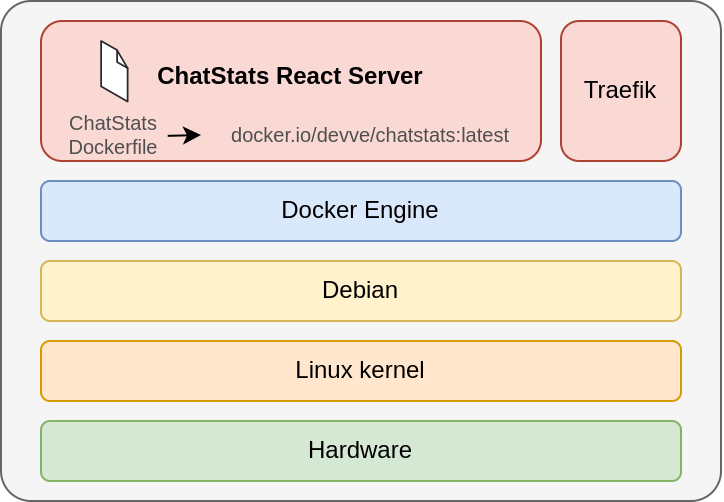
\includegraphics[width=0.6\textwidth]{img/server.png}
	\caption{Arquitectura en el servidor}
	\label{fig:chap4:architecture_server}
\end{figure}

Se ha decidido no instalar el software directamente sobre el sistema operativo, evitando problemas de dependencias y distintas versiones de las mismas para los componentes del sistema operativo. Asimismo, se evitan problemas de seguridad que puedan venir por vulnerabilidades en el código fuente y sus dependencias.

Hemos elegido virtualización ligera para ejecutar nuestro código en contenedores, por las razones que se exponen:

\begin{itemize}
	\item Se contienen las dependencias de terceros en una imagen.
	\item En caso de vulnerabilidad, solo se expone el contenedor y no el sistema completo.
	\item Los recursos se ocupan dinámicamente en función a las necesidades, al contrario que con la virtualización completa.
	\item Permite el despliegue en cualquier sistema operativo compatible con Linux, salvo arquitecturas ARM (que no es frecuente en servidores).
\end{itemize}

\subsection{ChatStats React Server}

Se trata del servidor de React que sirve el contenido. Tras construir la versión de producción con el código fuente, este contenedor sirve el contenido estático final, que enviará al cliente completamente cuando este solicite la aplicación web.

\subsection{Traefik}

Se ha decidido usar Traefik como \textit{proxy} inverso, que se sitúa frente al servidor de ChatStats para redirigir las peticiones realizadas a su contenedor correspondiente en el puerto adecuado.

Además, Traefik gestiona los certificados \acrshort{ssl} haciendo uso de \textit{Let's Encrypt}: autoridad sin ánimo de lucro que provee certificados para la capa \acrshort{tls} sin coste alguno.

\vspace{8mm}

Con todo, si en un futuro se quiere extender la arquitectura propuesta a un modelo de cliente-servidor; como en la tercera opción que se propone al comienzo de este capítulo, siempre se puede añadir un tercer contenedor en la última capa que implemente lógica adicional. Sería también necesaria cierta modificación en el código del cliente para implementar peticiones a este nuevo servicio.



\section{Arquitectura en el cliente}

A continuación se presenta la arquitectura que podemos encontrar en un cliente cualquiera.

\begin{figure}[H]
	\centering
	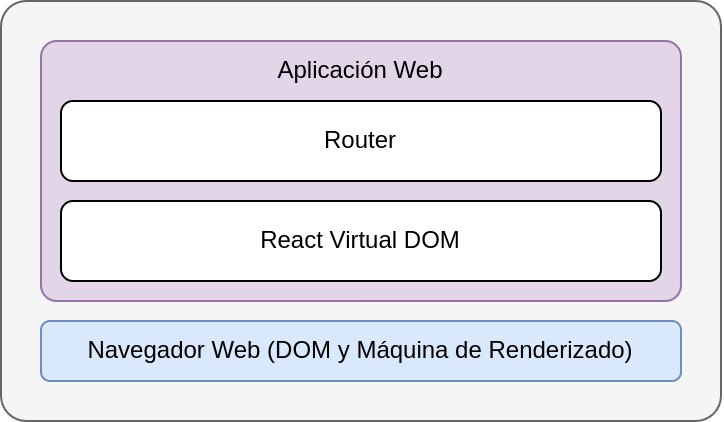
\includegraphics[width=0.6\textwidth]{img/client.png}
	\caption{Arquitectura en el cliente}
	\label{fig:chap4:architecture_client}
\end{figure}

\todi{Hacer esquinas del rectángulo menos redondeadas}

\subsection{Navegador}

El navegador juega un papel fundamental para el acceso y ejecución de cualquier aplicación web. Aunque no se entra en detalle en su estructura interna, sí que vamos a detallar la integración con \acrfull{pwa}. Esta integración que ofrecen algunos navegadores como los basados en Chromium, permite instalar aplicaciones web, con ventajas como:

\begin{itemize}
	\item La aplicación saldrá en el escritorio en teléfonos Android e iOS, así como en el cajón de aplicaciones del navegador.
	\item Posibilidad de acceso a notificaciones \textit{push} para el sistema (que no utilizaremos).
	\item Posibilidad de guardar en \textit{cache} el código del cliente, permitiendo su uso sin conexión a Internet.
\end{itemize}

Hay que mencionar también que Mozilla no ofrece soporte para \acrshort{pwa} en su navegador Firefox\cite{firefoxNoPWA}, aunque este puede ser habilitado mediante una extensión\cite{firefoxPWAextension}.

\subsection{Aplicación Web}

Es la última capa, se encuentra nuestra aplicación, cuya arquitectura de procesamiento se explica en la \autoref{chap:architecture:processing}. Explicamos a continuación los componentes lógicos que se encuentran en el cliente:

\subsubsection{Router}

ChatStats es una aplicación multipágina. Esto quiere decir que cuenta con diferentes rutas web en las que se muestran diferentes páginas. La página principal consolida la ruta `\textit{/}', mientras que `\textit{/graphs}' enruta la página para la visualización de los gráficos.

\subsubsection{React Virtual DOM}

El DOM virtual es un concepto de programación en el que una representación virtual de la interfaz de usuario (UI) es guardada en memoria y sincronizada con el DOM del navegador. Esto nos permite definir qué queremos en la interfaz de usuario y React conseguirá que el DOM virtual y el DOM del navegador se sincronicen.


\newpage
